% Created 2019-06-27 木 15:54
% Intended LaTeX compiler: pdflatex
\documentclass{article}

\usepackage{authblk}
\usepackage{graphicx}

\date{}
% \title{Core Challenge 2022: Graph Track Documentation}
\title{Every House on the Block: A generalized solution to creating ISR instances of large plan length}
\pagenumbering{gobble}

\author[1]{Remo Christen}
\author[1]{Salomé Eriksson}
\author[2]{Michael Katz}
\author[3]{Emil Keyder}
\author[4]{Christian Muise}
\author[4]{Alice Petrov}
\author[1]{Florian Pommerening}
\author[5]{\\ Jendrik Seipp}
\author[1]{Silvan Sievers}
\author[6]{David Speck}

\affil[1]{University of Basel}
\affil[2]{IBM T.J. Watson Research Center}
\affil[3]{Invitae}
\affil[4]{Queen's University}
\affil[5]{Linköping University}
\affil[6]{University of Freiburg}

\begin{document}
\maketitle

% -------------------------------------------------------------------

\section{Introduction}

Several strategies were tried throughout the course of the contest. From hand-crafted examples to exhaustive enumeration of smaller graphs with the aid of SAT solvers and knowledge compilers. Ultimately, a useful pattern for repeated movements was discovered. Since it is readily scalable, this is what is used for the submission. Throughout the remainder of the document, we describe the core concepts that make up the graph.

% -------------------------------------------------------------------

\section{The ``House'' Widget}

\begin{figure}[ht]
\centering
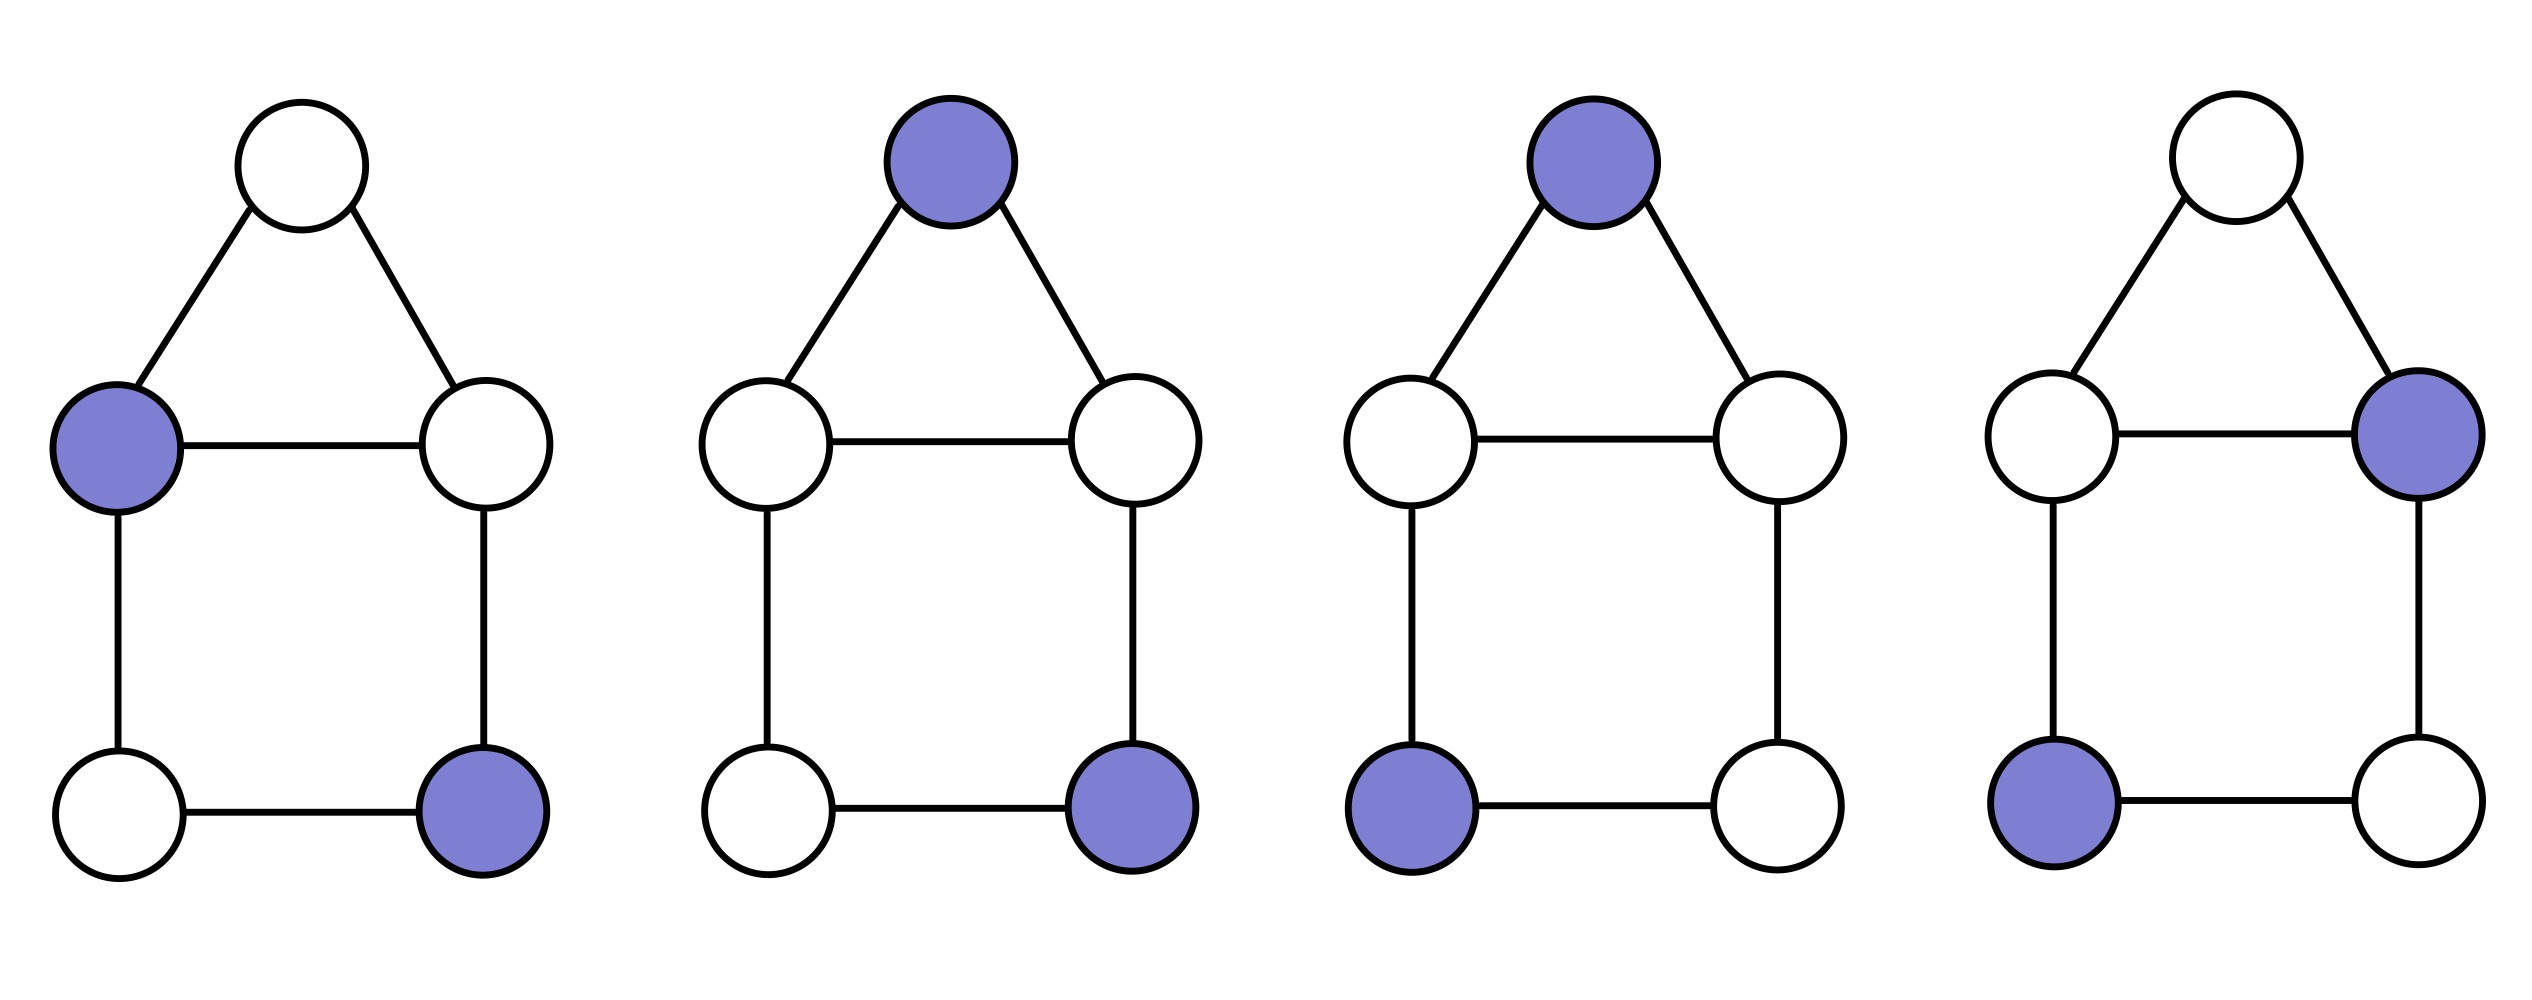
\includegraphics[width=0.8\textwidth]{house-widget.jpg}
\caption{\label{fig:house-widget}Reconfiguration sequence from ``off'' to ``on''}
\end{figure}

In order to encode bit flips in a graph, we leverage a five node subgraph we call the ``house widget'': a 4-cycle with two adjacent nodes leading to a 5th (essentially, a triangle sitting on top of a square). The house widget has a number of properties that make it ideal to use as a building block in creating exponential sequences.

\begin{enumerate}
\item The graph has an optimal ``long'' shortest reconfiguration sequence for ISR instances of order 5. 
\item You can only place two tokens on this widget, meaning each step of the reconfiguration sequence consists of a maximum independent set. In other words, the sequence is ``tight'' and no additional nodes can be added to the independent set at any point.
\item  The topmost node, which we call the ``anchor'', is occupied throughout the entire sequence with the exception of the starting state and ending state, and is required to switch the corners that the two tokens are on.
\item The sequence is unique. Thus, the solution space is a path and the behaviour of the widget is predictable.
\end{enumerate}

In summary, we have a widget that remembers its setting, takes five nodes to do so, and three moves to make it happen. We call one setting ``on'' and the other setting ``off'' (they're symmetric).

% -------------------------------------------------------------------

\section{Connecting Anchors}

\begin{figure}[ht]
\centering
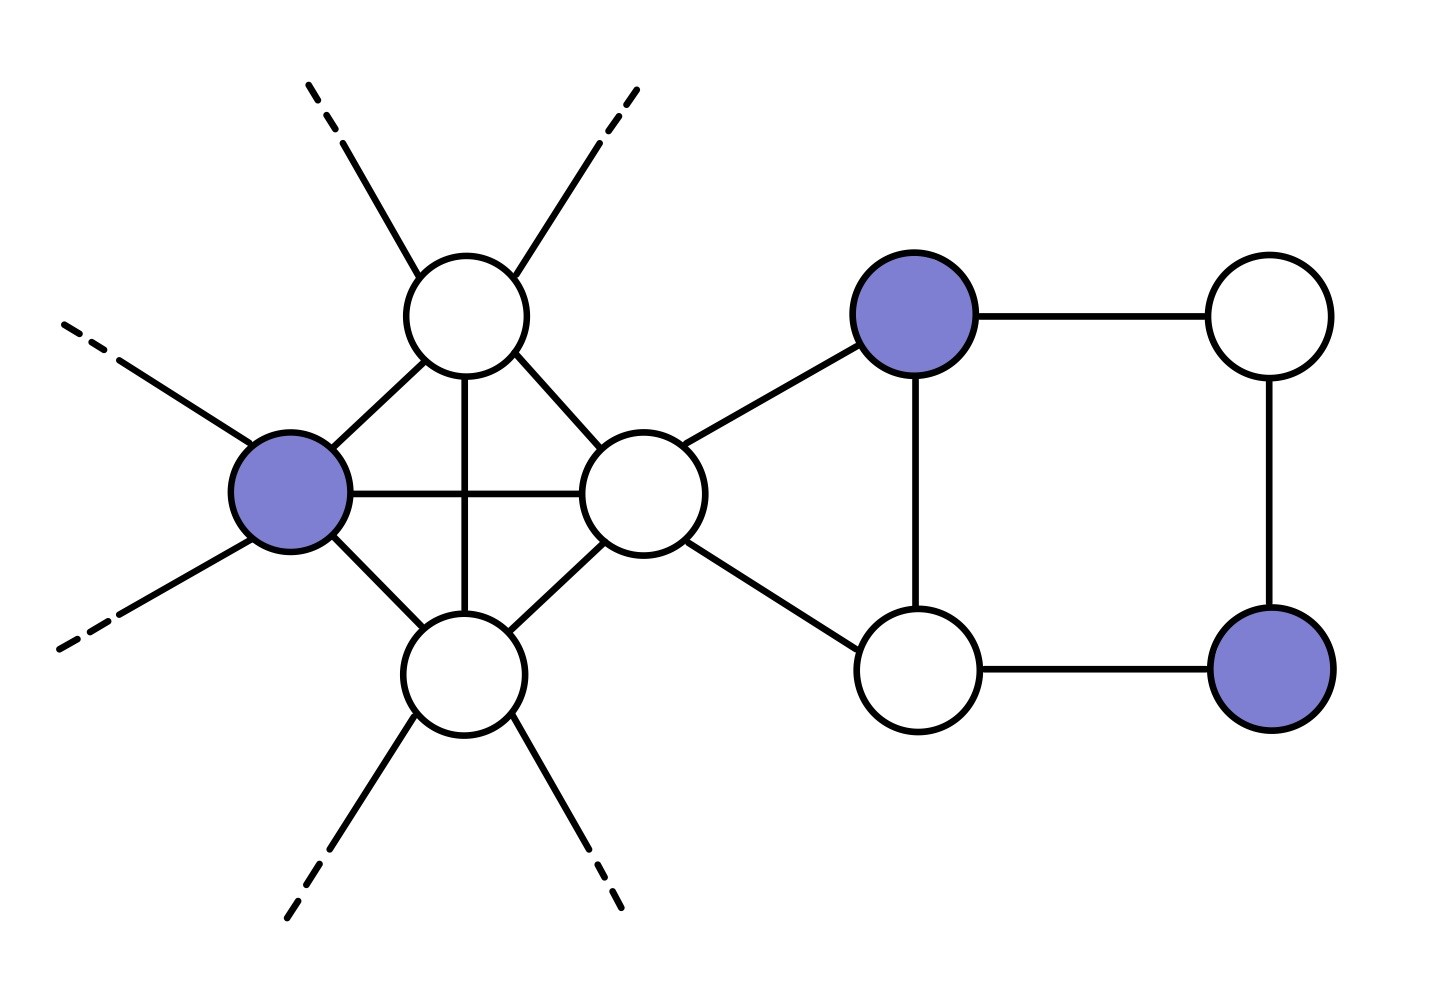
\includegraphics[width=0.6\textwidth]{connected-anchors.jpg}
\caption{\label{fig:connected-anchors}Four connected anchors; clearly, only one house can ``flip'' at a time}
\end{figure}

Since we treat our house widgets as bit flips, the first step in establishing an optimally long sequence is ensuring at most one house can be switching states at any given time. This is done by fully connecting the anchors of all houses in our graph. Recall that the anchor is both required to switch a house from ``on'' to ``off'' and is occupied throughout the sequence. By making the anchors a fully connected subgraph, we guarantee no houses switch states simultaneously.

% -------------------------------------------------------------------

\section{Flipping Bits}

\begin{figure}[ht]
\centering
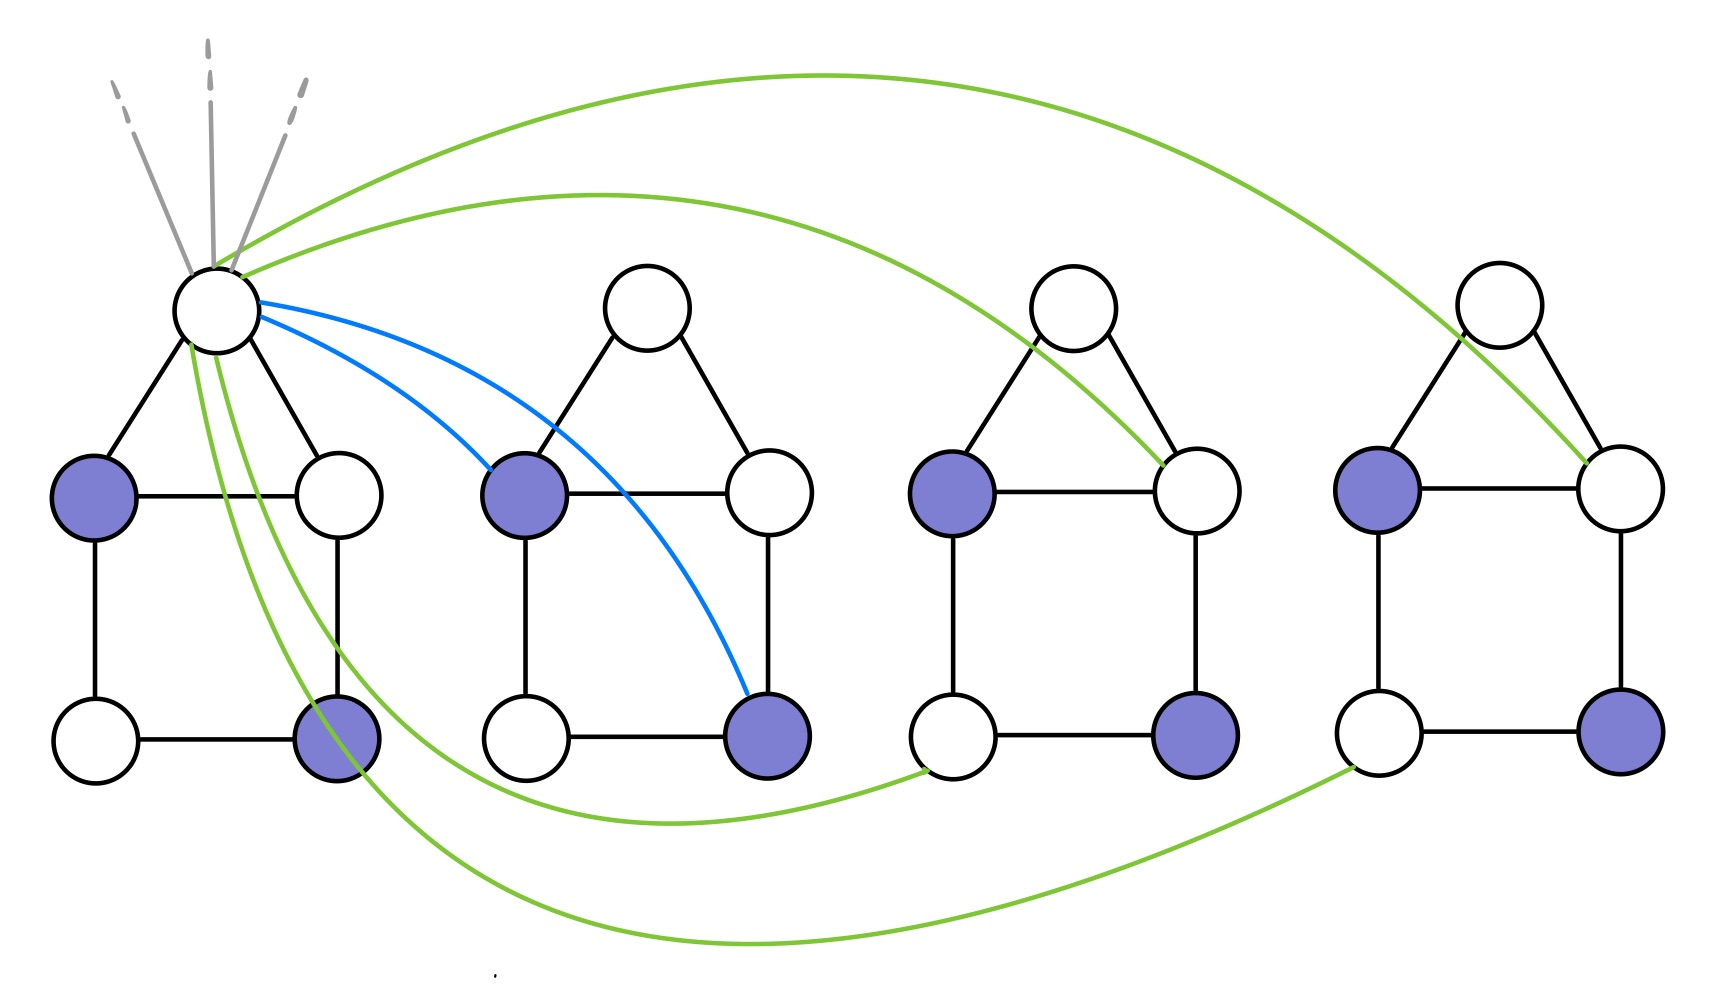
\includegraphics[width=0.8\textwidth]{flipping-bits-v1.jpg}
\caption{\label{fig:flipping-bits-v1}Edges for a single house. Blue and green edges correspond to Rules 1 and 2 respectively. Grey edges correspond to connections with other anchors.}
\end{figure}

\begin{figure}[ht]
\centering
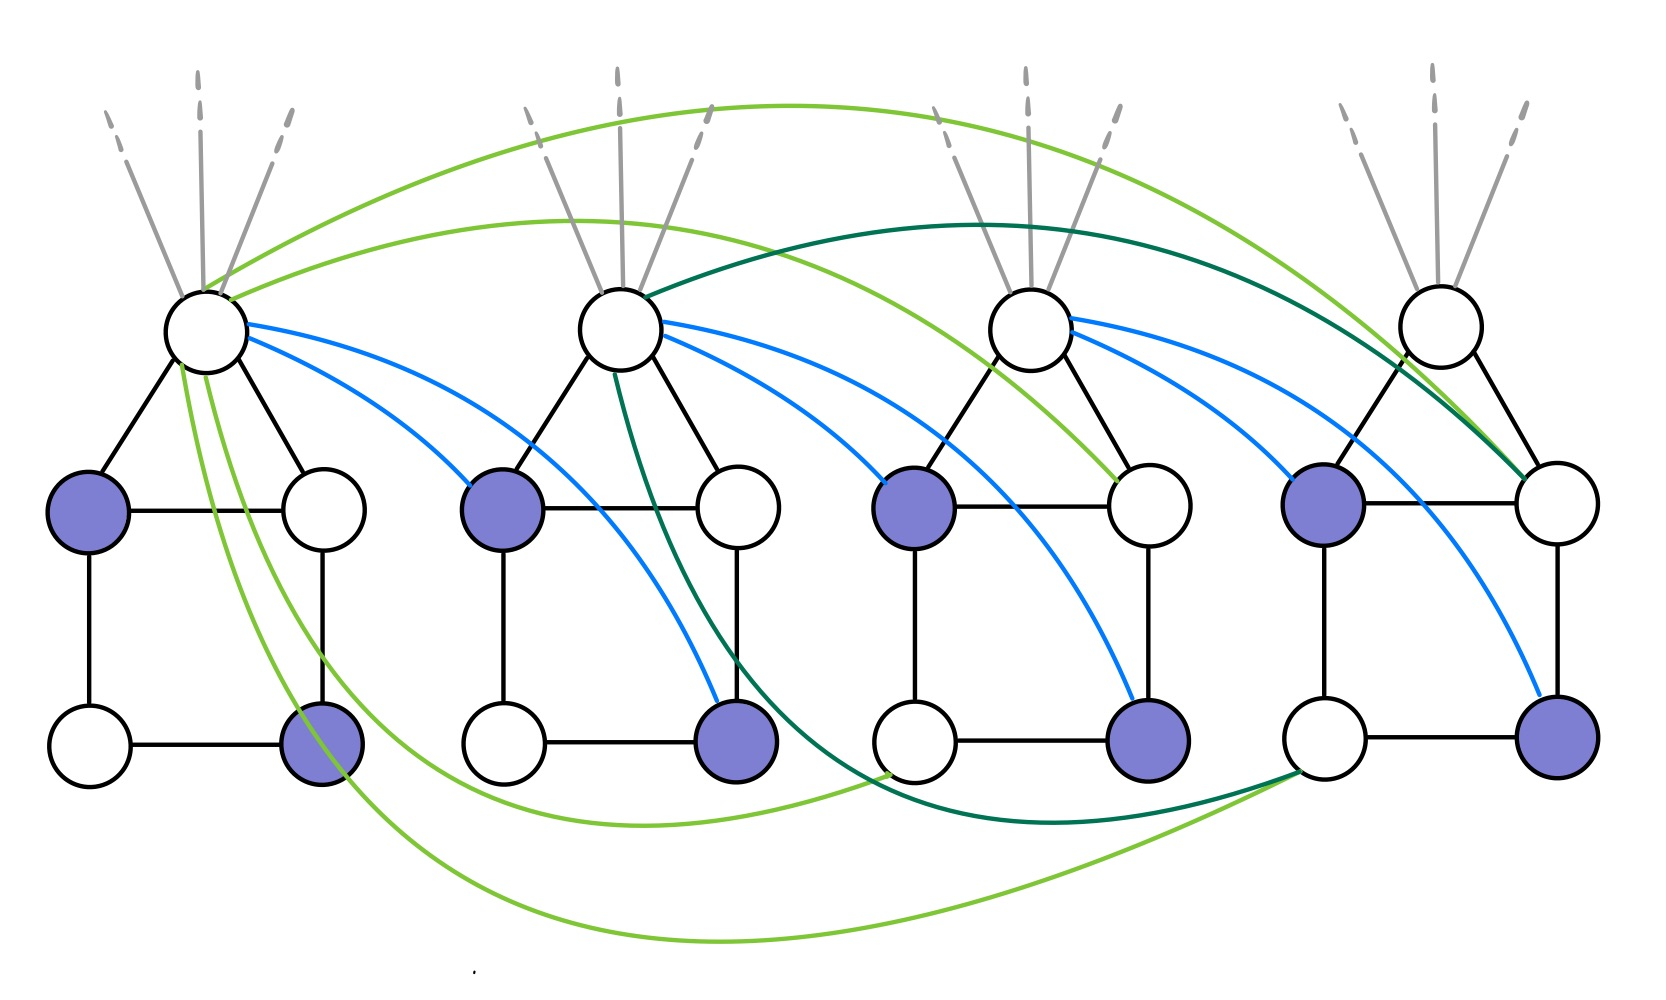
\includegraphics[width=0.8\textwidth]{flipping-bits-v2.jpg}
\caption{\label{fig:flipping-bits-v2}Four connected houses. Blue and green edges correspond to Rules 1 and 2 respectively. Assume all anchors are fully connected.}
\end{figure}

Now that we have a rigid set of widgets (referred to henceforth as bits) which we can turn ``on'' and ``off'', we must connect them in a manner that results in exponential growth. Assume bits are ordered (so there is a 1st bit, 2nd bit, etc..). The key challenge is that any edge between house bases will permanently rule out a pair of bit configurations, thus all additional inter-house edges are between an anchor and bit values of another house. The order of bit flips is then enforced by the following relations in order to flip bit $k$.

\begin{enumerate}
\item [Rule 1: ] Bit $k+1$ must be ``on''.
\item [Rule 2: ] Bits $k+2 \cdots n$ must all be ``off''.
\end{enumerate}

This sequence results in an exponential cost flipping things back and forth in order to get a low bit flipped.

\section{Generating Graphs}

\begin{figure}[ht]
\centering
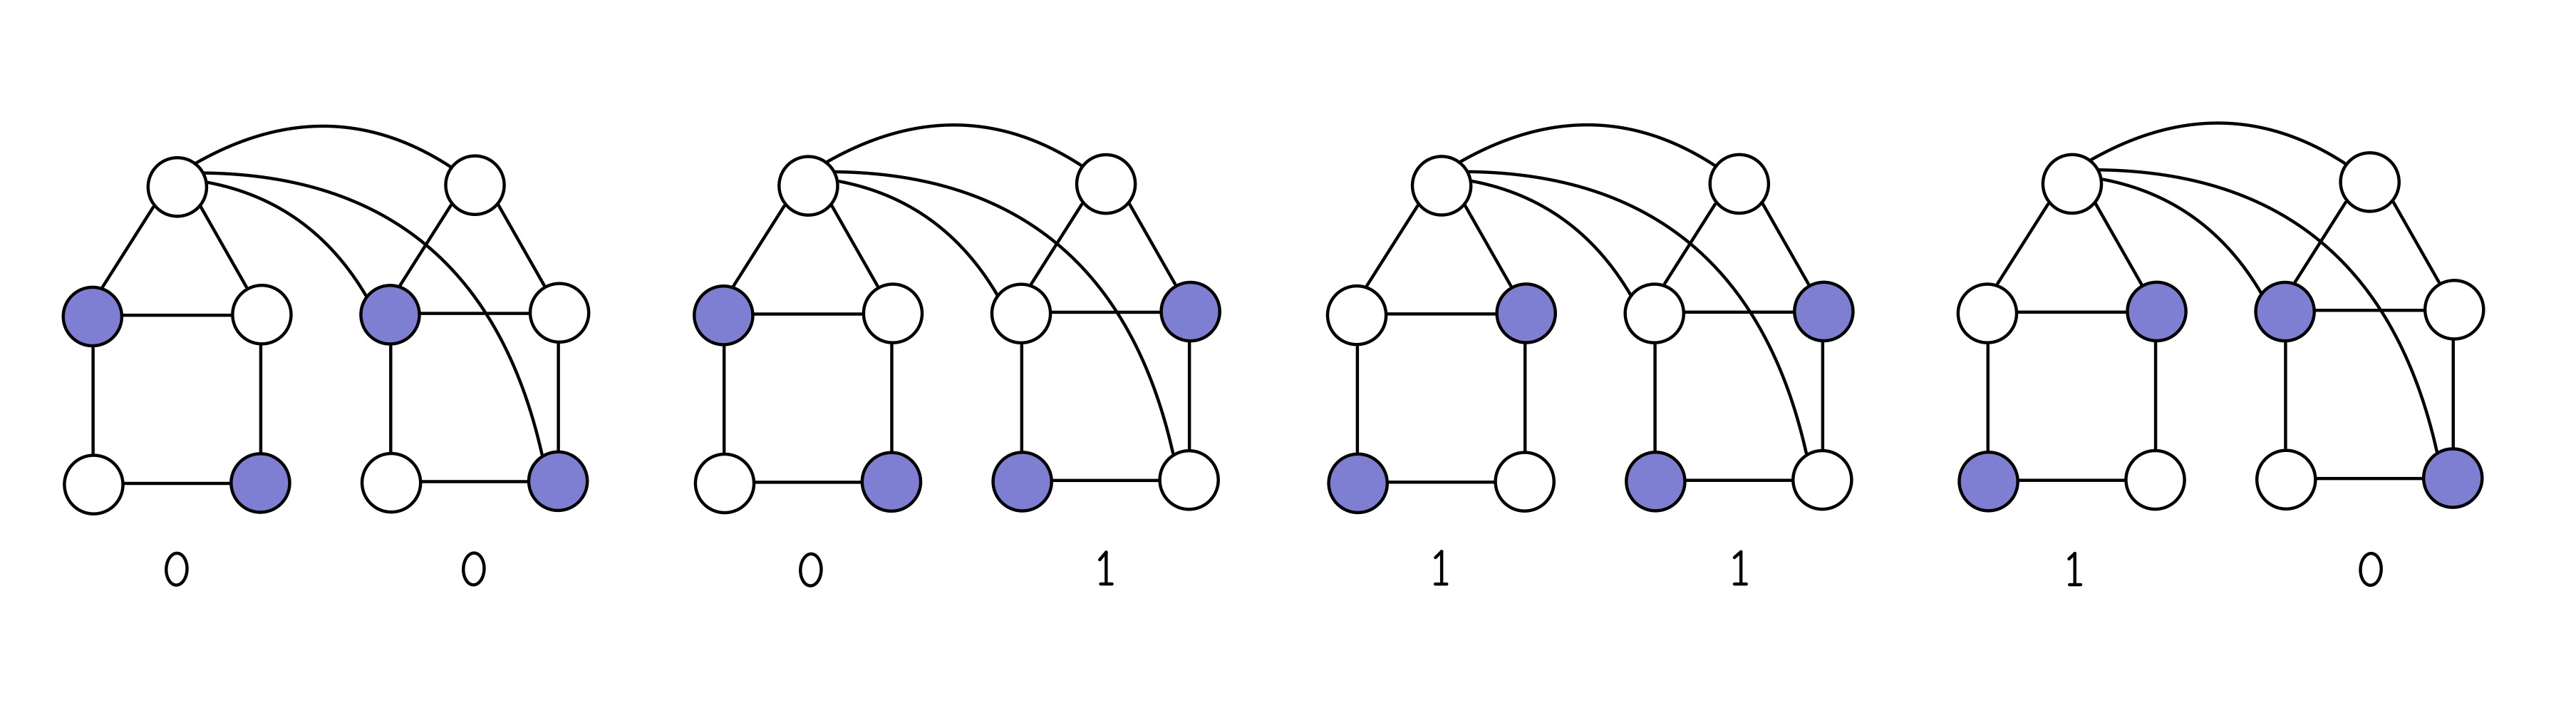
\includegraphics[width=1.0\textwidth]{generating-graphs.jpg}
\caption{\label{fig:generating-graphs}A series of bit flips for a graph of order 10. Note that each bit flip takes 3 moves, so the entire sequence is of length 9.}
\end{figure}

Putting everything together, graphs are generated as follows:

\begin{enumerate}
\item Create k ``houses''
\item Make the anchors of each house a fully connected subgraph of order k
\item Add edges corresponding to the three bit flipping rules listed in Section 4, \textit{Flipping Bits}
% \item Start with all houses off and end with all houses on # I believe this was deprecated in favor of using a planner to find better start/end states
\end{enumerate}

% -------------------------------------------------------------------

\section{Adding Widgets}

The final step is the strategy for adding an extra house. Suppose we have a sequence of k houses generated via the strategy above. We add house k+1 according to the following:

\begin{enumerate}
\item We can only flip house k+1 when the goal of house k is satisfied.
\item The new goal is the initial state of the k house sequence, combined with the flip of house k+1
\end{enumerate}

This forces the plan length to double with each new house: achieve the old goal of the k house sequence, flip house k+1, go back to the initial state of the k house sequence.

\section{Contest Instances}

Since each size was a multiple of 5, the submissions for the graph track take 2, 10, and 20 houses respectively for graphs of order n=10, 50, and 100.

The lengths of the optimal plans found are as follows:

\vspace{1em}

\begin{center}
\begin{tabular}{rl}
    $n$ & Length \\[0.5em]
    \hline \\
    10  & 9 \\[0.5em]
    50  & 3,069 \\[0.5em]
    100 & 3,145,725
\end{tabular}
\end{center}

% -------------------------------------------------------------------

\end{document}
